\documentclass[11pt]{article}
\usepackage{lmodern}
\usepackage[T1]{fontenc}
\usepackage[utf8]{inputenc}
\usepackage{fontspec}
\setmonofont{Source Code Pro}


\newif\ifslow\slowfalse %\slowtrue
\ifslow
  \usepackage[english]{babel}
  \usepackage[babel=true]{microtype}
\fi
\usepackage[top=1in, bottom=1in, left=1.25in, right=1.25in]{geometry}

\usepackage[backend=biber]{biblatex}
\bibliography{bib}

\newcommand{\bdia}{\blacklozenge}
\newcommand{\dia}{\Diamond}
\newcommand{\injR}{\texttt{injR}}
\newcommand{\injL}{\texttt{injL}}


\makeatletter%
\@ifundefined{basedir}{%
\newcommand\basedir{}%
}{}%
\makeatother%
%%%%%%%%%%%%%%%%%%%%%%%%%%%%%%%%%%%%%%%%%%%%%%%%%%%%%%%%%%%%%%%%
%% PACKAGES
%%%%%%%%%%%%%%%%%%%%%%%%%%%%%%%%%%%%%%%%%%%%%%%%%%%%%%%%%%%%%%%%

%\usepackage{amsmath}
\usepackage{amsfonts}
\usepackage{amsthm}
\usepackage{amssymb}
\usepackage{stmaryrd}

\usepackage{\basedir mathpartir}

\usepackage{\basedir pftools}
\usepackage{\basedir iris}

\usepackage{xcolor}  % for print version

\usepackage{graphicx}
\usepackage{enumitem}
\usepackage{semantic}
\usepackage{csquotes}

\usepackage{hyperref}

%%%%%%%%%%%%%%%%%%%%%%%%%%%%%%%%%%%%%%%%%%%%%%%%%%%%%%%%%%%%%%%%
%% SETUP
%%%%%%%%%%%%%%%%%%%%%%%%%%%%%%%%%%%%%%%%%%%%%%%%%%%%%%%%%%%%%%%%
\SetSymbolFont{stmry}{bold}{U}{stmry}{m}{n} % this fixes warnings when \boldsymbol is used with stmaryrd included

\extrarowheight=\jot	% else, arrays are scrunched compared to, say, aligned
\newcolumntype{.}{@{}}
% Array {rMcMl} modifies array {rcl}, putting mathrel-style spacing
% around the centered column. (We used this, for example, in laying
% out some of Iris' axioms. Generally, aligned is simpler but aligned
% does not work in mathpar because \\ inherits mathpar's 2em vskip.)
% The capital M stands for THICKMuskip. The smaller medmuskip would be
% right for mathbin-style spacing.
\newcolumntype{M}{@{\mskip\thickmuskip}}

\definecolor{StringRed}{rgb}{.637,0.082,0.082}
\definecolor{CommentGreen}{rgb}{0.0,0.55,0.3}
\definecolor{KeywordBlue}{rgb}{0.0,0.3,0.55}
\definecolor{LinkColor}{rgb}{0.55,0.0,0.3}
\definecolor{CiteColor}{rgb}{0.55,0.0,0.3}
\definecolor{HighlightColor}{rgb}{0.0,0.0,0.0}

\definecolor{grey}{rgb}{0.5,0.5,0.5}
\definecolor{red}{rgb}{1,0,0}

\hypersetup{%
  linktocpage=true, pdfstartview=FitV,
  breaklinks=true, pageanchor=true, pdfpagemode=UseOutlines,
  plainpages=false, bookmarksnumbered, bookmarksopen=true, bookmarksopenlevel=3,
  hypertexnames=true, pdfhighlight=/O,
  colorlinks=true,linkcolor=LinkColor,citecolor=CiteColor,
  urlcolor=LinkColor
}


%\theoremstyle{definition}
%\newtheorem{prop}{Prop}
\newtheorem{defn}{Definition}
\newtheorem{cor}{Corollary}
\newtheorem{conj}{Conj}
\newtheorem{lem}{Lemma}
\newtheorem{thm}{Theorem}

\newtheorem{exercise}{Exercise}

%%%%%%%%%%%%%%%%%%%%%%%%%%%%%%%%%%%%%%%%%%%%%%%%%%%%%%%%%%%%%%%%
%% GENERIC MACROS
%%%%%%%%%%%%%%%%%%%%%%%%%%%%%%%%%%%%%%%%%%%%%%%%%%%%%%%%%%%%%%%%
\newcommand*{\Sref}[1]{\hyperref[#1]{\S\ref*{#1}}}
\newcommand*{\secref}[1]{\hyperref[#1]{Section~\ref*{#1}}}
\newcommand*{\lemref}[1]{\hyperref[#1]{Lemma~\ref*{#1}}}
\newcommand{\corref}[1]{\hyperref[#1]{Cor.~\ref*{#1}}}
\newcommand*{\defref}[1]{\hyperref[#1]{Definition~\ref*{#1}}}
\newcommand*{\egref}[1]{\hyperref[#1]{Example~\ref*{#1}}}
\newcommand*{\appendixref}[1]{\hyperref[#1]{Appendix~\ref*{#1}}}
\newcommand*{\figref}[1]{\hyperref[#1]{Figure~\ref*{#1}}}
\newcommand*{\tabref}[1]{\hyperref[#1]{Table~\ref*{#1}}}

\newcommand{\changes}{{\bf\color{red}{Changes}}}
\newcommand{\TODO}{\vskip 4pt {\color{red}\bf TODO}}


\newcommand{\ie}{\emph{i.e.,} }
\newcommand{\eg}{\emph{e.g.,} }
\newcommand{\etal}{\emph{et~al.}}
\newcommand{\wrt}{w.r.t.~}

\newcommand{\aaron}[1]{{\color{red}\textbf{AT: #1}}}
\newcommand{\derek}[1]{{\color{red}\textbf{DD: #1}}}
\newcommand{\lars}[1]{{\color{red}\textbf{LB: #1}}}
\newcommand{\kasper}[1]{{\color{red}\textbf{KS: #1}}}
\newcommand{\ralf}[1]{{\color{red}\textbf{RJ: #1}}}
\newcommand{\dave}[1]{{\color{red}\textbf{PDS: #1}}}
\newcommand{\hush}[1]{}
\newcommand{\relaxguys}{%
	\let\aaron\hush%
	\let\derek\hush%
	\let\lars\hush%
	\let\kasper\hush%
	\let\ralf\hush%
	\let\dave\hush%
}


\begin{document}

\title{\bfseries iris-atomic}
\author{Zhen Zhang}
\maketitle

\section{Overview}

\begin{figure}[hb]
  \centering
  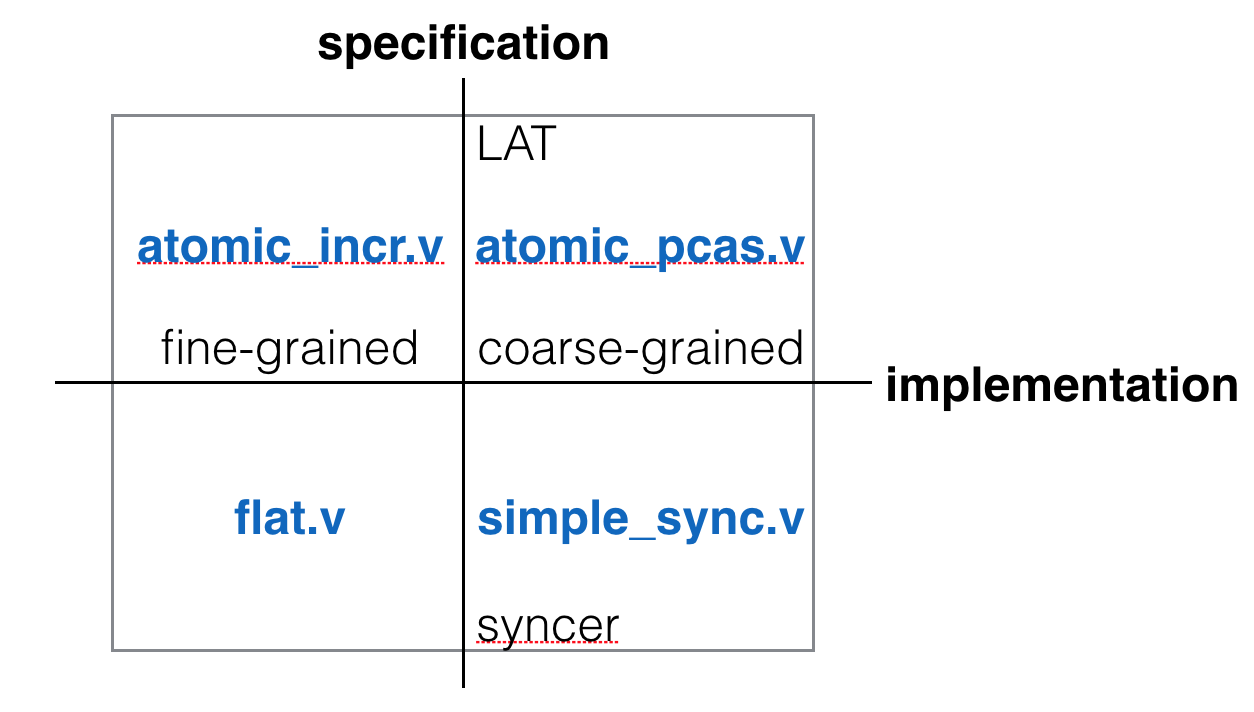
\includegraphics[width=0.5\textwidth]{ispace}
  \caption
   {Two dimensions of atomicity verification in Iris}
\end{figure}

\section{Generic syncer spec}

\begin{align*}
  \text{synced}(R, f', f) \eqdef
  \All P, Q, x.
    &\hoare{ R * P(x)}{f(x)}{ v.\,R * Q(x,v) } \ra \\
    &\hoare{ P(x)}{f'(x)}{ v.\,Q(x,v) }
\end{align*}

\[ \text{syncer}(R, s) \eqdef \All f. \wpre{s(f)}{ f'.\, \text{synced}(R, f', f)} \]


\[\text{mkSyncer}(f) \eqdef \All R. \hoare{R}{f()}{ s.\,\always \text{syncer}(R, s)} \]

This \textbf{generic syncer spec} is inspired by CaReSL. In CaReSL, fine-grained syncer (e.g. flat combiner) is proven to be contextual refinement of coarse-grained \texttt{mkSync} (See section \ref{mksync}). However, there is no program refinement yet in Iris, so I made this generalization and prove that flat combiner satisfies this \emph{directly}.

In fact, any sensible syncer is expected to satisfy this generic spec.

Besides generalization, I also split original spec into two parts, corresponding to two calls that happen at different times. More generally speaking, this problem is caused by a special case of curried function (e.g. $\lambda x_1.\, \lambda x_2.\,...$): Is it possible to go from \[\All x_1, x_2. \hoare{P(x_1, x_2)}{f(x_1, x_2)}{Q(x_1, x_2)}\] to \[\All x_1. \hoare{\top}{f(x_1)}{f_1.\, \All x_2. \hoare{P(x_1, x_2)}{f_1(x_2)}{Q(x_1, x_2)}}\], assuming that \(f \eqdef \lambda x_1, x_2.\, e\).

Finally, I'd like to point out that pre- and post-conditions $P, Q$ are universally qualified per application, that is to say, $P, Q$ are arbitrary depending on the context.

And similarly, $f$ is universally qualified per synchronization, which means that syncer is only parameterized by the shared resource $R$, it can work with any operation that needs to access this $R$.

\section{Logically atomic triple (LAT)}

\begin{align*}
    &\lahoare{g.\, \alpha(g)}{e}{v.\, \beta(g, v)}[E_i][E_o] \eqdef\\
    &\All P, Q.
    \begin{aligned}
          &P \vs[Eo][Ei] \Exists g, \alpha(g) * (\alpha(g) \vsW[Ei][Eo] P \land \All v. \beta(g, v) \vsW[Ei][Eo] Q(g, v)) \wand \\
          &\hoare{P}{e}{v.\, \Exists g. Q(g, v)}
    \end{aligned}
\end{align*}

Note again, the $P, Q$ are arbitrary depending on the context.

And also, note the separation product of two linear view shifts: First one represents \textbf{abandon} direction, while the second one represents \textbf{commit} direction. Using linear view shifts enables us to frame alongside the transition some non-persistent resource.

\begin{figure}[hb]
  \centering
  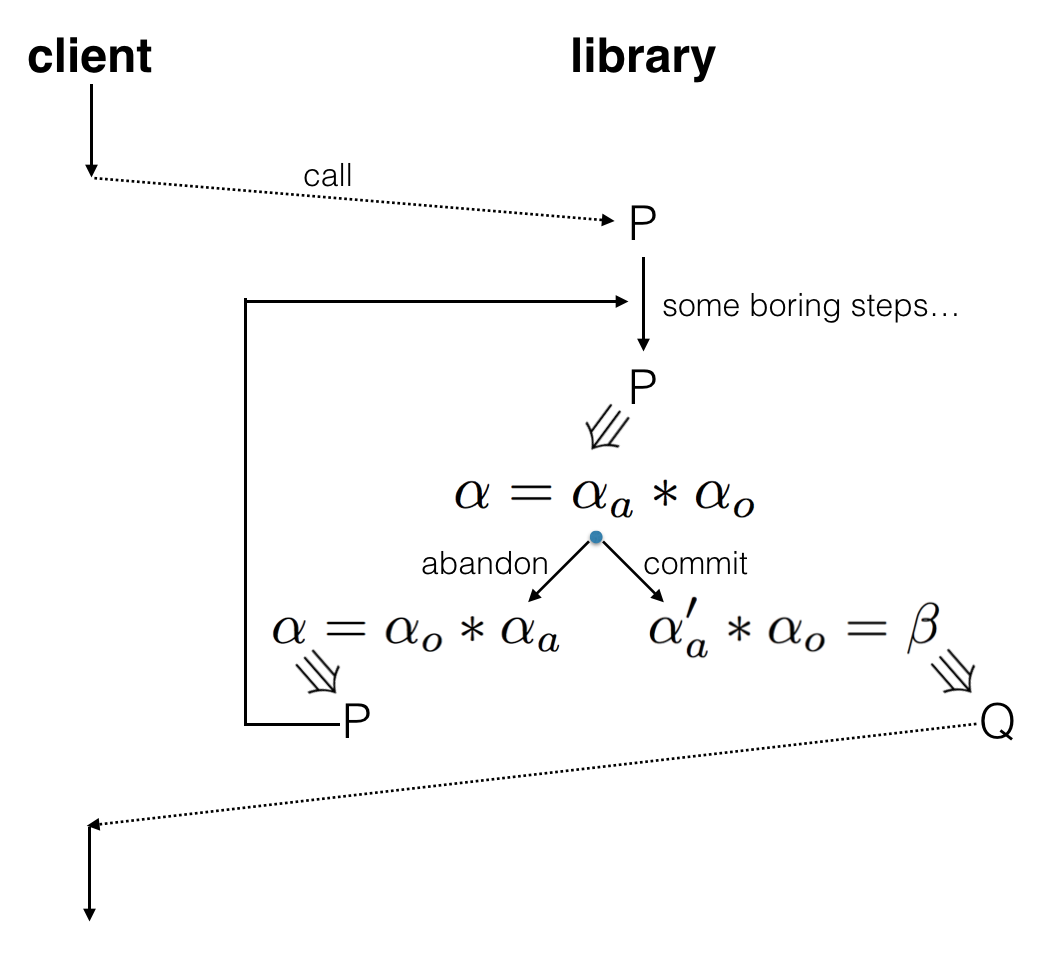
\includegraphics[width=0.5\textwidth]{lat}
  \caption
   {Sketch of how library function specified with LAT will be used}
\end{figure}

\section{Coarse-grained syncer}\label{mksync}

First, we give the CaReSL's \texttt{mkSync} written in heap-lang (which is basically the same as in Coq, despite a few cosmetics).

\begin{verbatim}
mk_sync :=
    λ: <>,
       let l := newlock() in
       λ: f x,
          acquire l;
          let ret := f x in
          release l;
          ret.
\end{verbatim}

Okay, now the question is: can we give a LAT spec for \texttt{mk\_sync}? Actually, we can! and we can do this in a general way (i.e. for any syncer satisfying the generic syncer spec). We will briefly discuss about it in the next section.

\section{Encoding generic syncer spec as a LAT-style spec}

The first question is: \textbf{Why do we want to do so?}

First, they both talk about atomicity, so we will naturally want to know what is the possible relationship between them. And second, the generic syncer spec is not canonical -- it doesn't tell explicitly what effects that operation has. When use the generic syncer spec as a client, you have to prove something about $e$ every time. But LAT, on the contrary, gives you the exact specification of the operation itself, which means that you only need to prove the viewshifts (in some sense similar to weakening/strengthening rules). And most importantly, this exact specification, should look exactly like the sequential specification! Just consider the following illustrative comparison of a sequential/concurrent stack \texttt{push} spec:

\begin{align*}
  \All xs.\hoare{stack(s, xs)}{\texttt{push}(x, s)}{\_.\, stack(s, x::xs)}\\
  \lahoare{xs.\, stack'(s, xs)}{\texttt{push'}(x, s)}{\_.\, stack'(s, x::xs)}
\end{align*}

The second question is: \textbf{Is it possible to do so?}

Intuitively, what syncer spec says is that the $e$'s sequential effects are \emph{compressed} to a single point. Consider the coarse-grained implementation of generic syncer spec, \texttt{mk\_sync}, it guards the resource $R$ by putting it inside a lock, thus every operation will exclusively own $R$ for a certain period, which makes the whole operation look atomic, when observed from outside in terms of resource accessing.

The third question is: \textbf{How to do it?}

First, consider what LAT's client can provide to the library: abandoning and committing viewshifts. And these two actions must happen instantly. So, naturally, we will try to commit at the time of finishing the operation and give back the $R$ to lock. But what about abandoning? What role will it have in the syncer spec?

Remember that there is a canonical pre-condition $\alpha$ in LAT, which should coincide with the sequential spec. But the sequential code, when executed between the lock/unlock, is still non-atomic. So after we exchange $P$ for $\alpha$, we must retain $\alpha$ for a long time, while we also have to close the LAT viewshifts in an instant. We can't close by abandoning, since we need to give back the $\alpha$; and we can't close by committing, since we haven't started the action yet!

But wait, why we \emph{must} give back $\alpha$ while losing it? What if we require that $\alpha$ is duplicable? Then problem solved! We just need to abandon in the beginning to get a duplicated $\alpha$ out, then committing with $P$ when finishing off.

Now, with a sketch in mind, I will introduce you to the detailed construction: First, here is the specialized logically atomic triple to serve this purpose:

\[ gtriple(\gname, \alpha, f, x, \beta, E_i, E_o) \eqdef
   \lahoare{g.\, \ownGhost{\gname}{g^{1/2}} * \always \alpha(g)}
           {f(x)}
           {v.\, \Exists g'. \ownGhost{\gname}{g'^{1/2}} * \beta(x, g, g', v)}[E_i][E_o]\]

Here, $g$ represents \textbf{ghost state}. $g$ can be of any proper type. $\ownGhost{\gname}{g'^{1/2}}$ is a snapshot of $g$, i.e. local knowledge about the physical configuration. (Why it is written in such way? Well, this is the implementation detail related to the monoid used to encode this).

Here, the persistent (thus duplicable) $\alpha(g)$ is some extra condition. And in the post condition, we say there exists an updated ghost state $g'$, which satisfy $\beta$, a relation over input, previous state, current state, and output.

Let's take concurrent \texttt{push} again as an example. If $s$ is a stack pointer, \[R_s \eqdef \Exists xs. stack(s, xs) * \ownGhost{\gname}{xs^{1/2}}\] is the physical configuration plus global snapshot, then $\text{synced}(stack(s, xs), \texttt{push'}, \texttt{push}(s))$ should expand like this:

\begin{align*}
  \All P, Q, x.
    &\hoare{ R_s * P(x)}{\texttt{push}(s)(x)}{ v.\,R_s * Q(x,v) } \ra \\
    &\hoare{ P(x)}{\texttt{push'}(x)}{ v.\,Q(x,v) }
\end{align*}

And the LAT we can get from it looks like this:

\[\lahoare{xs.\, \ownGhost{\gname}{xs^{1/2}}}{\texttt{push'}(x)}{\_.\, \Exists xs'. \ownGhost{\gname}{xs'^{1/2}} * (xs' = x::xs)} \]

Here, note that in this case $\always \alpha(g)$ is selected as $\top$ (thus we can imagine that in most cases persistent restriction is not much of a problem); also, $s$ is entirely hidden somewhere in some global place, i.e., using $\ownGhost{\gname}{xs^{1/2}}$, you can also atomically access $\Exists s. stack(s, xs)$, even though such accessing is not specified as a LAT.

Now, let's consider the last question: \textbf{How to formalize it?}

\begin{verbatim}
sync(mk_syncer) :=
  λ: f_seq l,
     let s := mk_syncer() in
     s (f_seq l).
\end{verbatim}

The code above is a helper function \texttt{sync}, which constructs the syncer, partially applies internal state value \texttt{l} to the sequential operation \texttt{f\_seq}, and synchronizes the partially applied operation. There is an assumption that \texttt{l} should represent a valid state (either freshly constructed or whatever).

Now, if conditions $seqSpec(\texttt{f\_seq}, \phi, \alpha, \beta, \top)$ (see \ref{seq}) and $mkSyncer(\texttt{mk\_syncer})$ are satisfied, then we have:

\[
\All g_0.
  \phi(l, g_0)
  \proves \wpre{\texttt{sync}(\texttt{mk\_syncer}, \texttt{f\_seq}, l)}{ f.\,
    \Exists \gname. \ownGhost{\gname}{g_0^{1/2}} *
    \All x. \always gtriple(\gname, \alpha, f, x, \beta, E_i, \top)}
\]

Here is the definition of sequential specification pattern \label{seq}:

\[seqSpec(f, \phi, \alpha, \beta, E) \eqdef
      \All l.
         \hoare{\top}{f(l)}{f'.\,
            \begin{aligned}
            \pure &\All x, \Phi, g.\\
                &\phi (l, g) * \always \alpha(g) *\\
                &(\All v, g'. \phi(l, g') \wand \beta(x, g, g', v) \vsW[E][E] \Phi(v))\\
                &\proves \wpre{f'(x)}[E]{ \Phi }
              \end{aligned}
        }\]

In pre-condition, we have persistent $\alpha(g)$ and exclusive ownership of shared state; and when it returns, we get back the updated physical state $g'$, as well as $\beta$.

Funny thing is again that I have to apply $f$ to $l$ first ... because of currying problem.

To be more concrete, here is the invariant that will be used globally: \( (\Exists g. \phi(l, g') * \ownGhost{\gname}{g^{1/2}} * P x \).

\begin{figure}[hb]
  \centering
  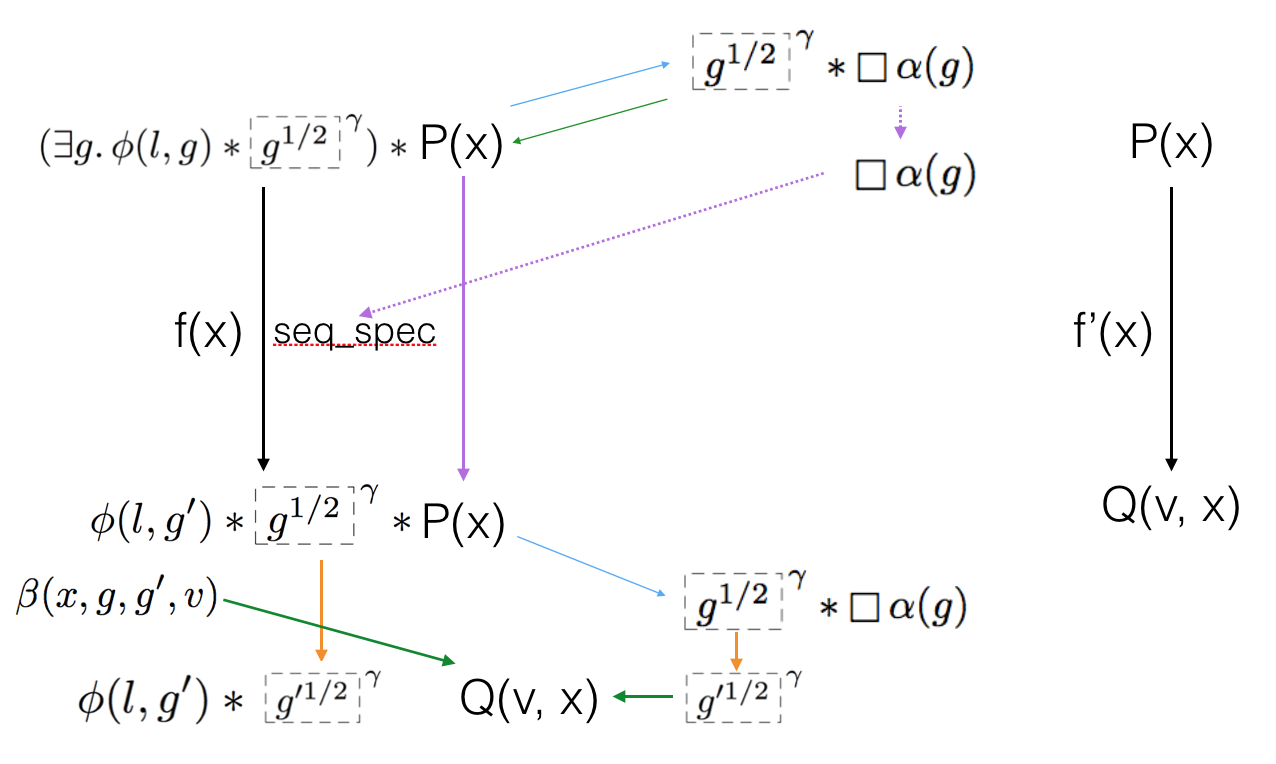
\includegraphics[width=0.5\textwidth]{atomic_sync}
  \caption{The sketch of proof: to prove triple for \texttt{f'(x)}, we prove another one for \texttt{f(x)}.
           The blue lines are opening viewshifts; the green lines are closing viewshifts; the orange lines are ghost update }
\end{figure}

\section{Treiber's stack}

\begin{verbatim}
push s x :=
  let hd := !s in
  let s' := ref SOME (x, hd) in
  if CAS s hd s'
    then ()
    else push s x.

pop s :=
  let hd := !s in
  match !hd with
  | SOME (x, hd') =>
    if: CAS s hd hd'
      then SOME x
      else pop s
  | NONE => NONE
  end.

iter hd f :=
  match !hd with
  | NONE => ()
  | SOME (x, hd') => f x ; iter hd' f
  end.

\end{verbatim}

These \texttt{push} and \texttt{pop} are all standard lock-free implementations. We will give LAT spec for these two operations first:

\subsection{Logically atomic spec (version 1)}

\[ \lahoare{xs.\, stack(s, xs)}{push(s, x)}{stack(s, x::xs)}[heapN][\top]\]
\[ \lahoare{xs.\, stack(s, xs)}{pop(s)}{v. \begin{split} (&\Exists x, xs'. v = SOME(x) * stack(s, xs')) \lor\\
                                            (&v = NONE * xs = \emptyset * stack(s, \emptyset)) \end{split}}[heapN][\top]\]


\subsection{Logically atomic spec (version 2)}

\[ \lahoare{hd, xs.\, s \mapsto hd * list(hd, xs)}{push(s, x)}{\Exists hd'. s \mapsto hd' * hd' \mapsto SOME(x, hd) * list(hd, xs)}[heapN][\top]\]
\[ \lahoare{hd, xs.\, s \mapsto hd * list(hd, xs)}{pop(s)}{v.
    \begin{split}
      (&\Exists x, xs', hd'.
          \begin{aligned}
            &v = SOME(x) * hd \mapsto SOME(x, hd') *\\
            &s \mapsto hd' * list(hd', xs')
          \end{aligned})\lor\\
      (&v = NONE * xs = \emptyset * hd \mapsto NONE)
    \end{split}
  }[heapN][\top]
  \]

\subsection{Why such dichotomy?}
Apparently, the version 1 is more preferable as a general spec, since the implementation might not necessarily be a linked-list.

But if we want to iterate over it using \texttt{iter} using a per-item style spec, than we might expose enough implementation details to tie per-item resource to physical location. And as a result, to maintain such property, we must also make \texttt{push}'s LAT spec exposing enough details as well (And it doesn't even make sense to use \texttt{pop} in this case). Below is the discussion about per-item spec.

\section{Per-item spec}

\begin{align*}
  fSpec &(\gname, xs, s, f, Rf, RI) \eqdef\\
    &\All x.
      \hoare{(\Exists hd. evs(\gname, hd, x)) * \knowInv\iname{\Exists xs. stack'(\gname, xs, s) * RI} * Rf}{f(x)}{ v.\, v = () * Rf}
\end{align*}

The $fSpec$ specifies that $f$ can access the per-item resource predicate associated with $x$ through open/close the global invariants. The $evs(\gname, hd, x)$ provides the \emph{evidence} that $x$ is part of the stack.

The first $\exists hd$ can be interpreted as ``We don't care which cell pointer points to the item $x$ in stack"; The second $\exists xs$ can be interpreted as ``We don't care what $s$ is \emph{currently} pointing to, since the previously existing elements still exist in the stack now".

Now, let's observe the \texttt{iter}'s spec and \texttt{push}'s spec (in a per-item setting):

\begin{align*}
  iterSpec&(\gname, s, Rf, RI) \eqdef\\
    &\All xs, hd, f.\\
         &fSpec(\gname, xs, s, f, Rf, RI) \ra\\
         &\hoare{\knowInv\iname{\Exists xs. stack'(\gname, xs, s) * RI} * list'(\gname, hd, xs) * Rf}{iter(hd, f)}{ v.\, v = () * Rf}
\end{align*}

\begin{align*}
  pushSpec&(\gname, s, x, RI) \eqdef\\
  &\hoare{R(x) * \knowInv\iname{\Exists xs. stack'(xs, s) * RI}}{push(s, x)}{v.\, v = () * (\Exists hd. ev(\gname, hd, x))}
\end{align*}

Okay, back to the per-item spec, why do you need to make sure that the stack is growth-only, and governed by a global invariant?

Answer: because we need to iterate thought it non-atomically. I mean, the process of iteration is not atomic. The single operation f still needs to atomically access any resource related x.

However, my current $fSpec$ is quite bad actually ... first, CaReSL has a smaller, nicer per-item spec; second, it doesn't sound perfectly legitimate that we can't pop things out ... I just need to make sure that the things \emph{currrently in} the stack conforms to certain resource predicate. So, if the structure of linking allows us to control validities of all possible references into certain item, then popping out an element can be atomic, thus doesn't compromise the basic invariant.

\section{Flat combiner}

Here is my implementation:

\begin{verbatim}
doOp :=
  λ: p,
     match !p with
     | InjL (f, x) => p <- InjR (f x)
     | InjR _ => ()
     end.

try_srv :=
  λ: lk s,
    if try_acquire lk
      then let hd := !s in
           iter hd doOp;
           release lk
      else ().

loop p s lk :=
    match !p with
    | InjL _ =>
        try_srv lk s;
        loop p s lk
    | InjR r => r
    end.

install :=
  λ: f x s,
     let p := ref (InjL (f, x)) in
     push s p;
     p.

mk_flat :=
  λ: <>,
   let lk := newlock() in
   let s := new_stack() in
   λ: f x,
      let p := install f x s in
      let r := loop p s lk in
      r.
\end{verbatim}

Compared to CaReSL, here are several notable differences:

\begin{itemize}
\item I break them down into five procedures, instead of nesting them inside the constructor. They all have their own spec, and it is easier to reason about.
\item CaReSL’s flat constructor takes \texttt{f}; mine doesn’t, which is more flexible.
\item CaReSL’s install utilizes TLS (thread-local storage) to avoid severe memory leakage. In my implementation, a new slot is created and pushed every time the operation is called. It is terrible in practice, but nevertheless follows the same spec.
\end{itemize}

Also, another problem that exists both in my, CaReSL, and FCSL’s example code, is that we never recycle the slots.

\begin{figure}[hb]
  \centering
  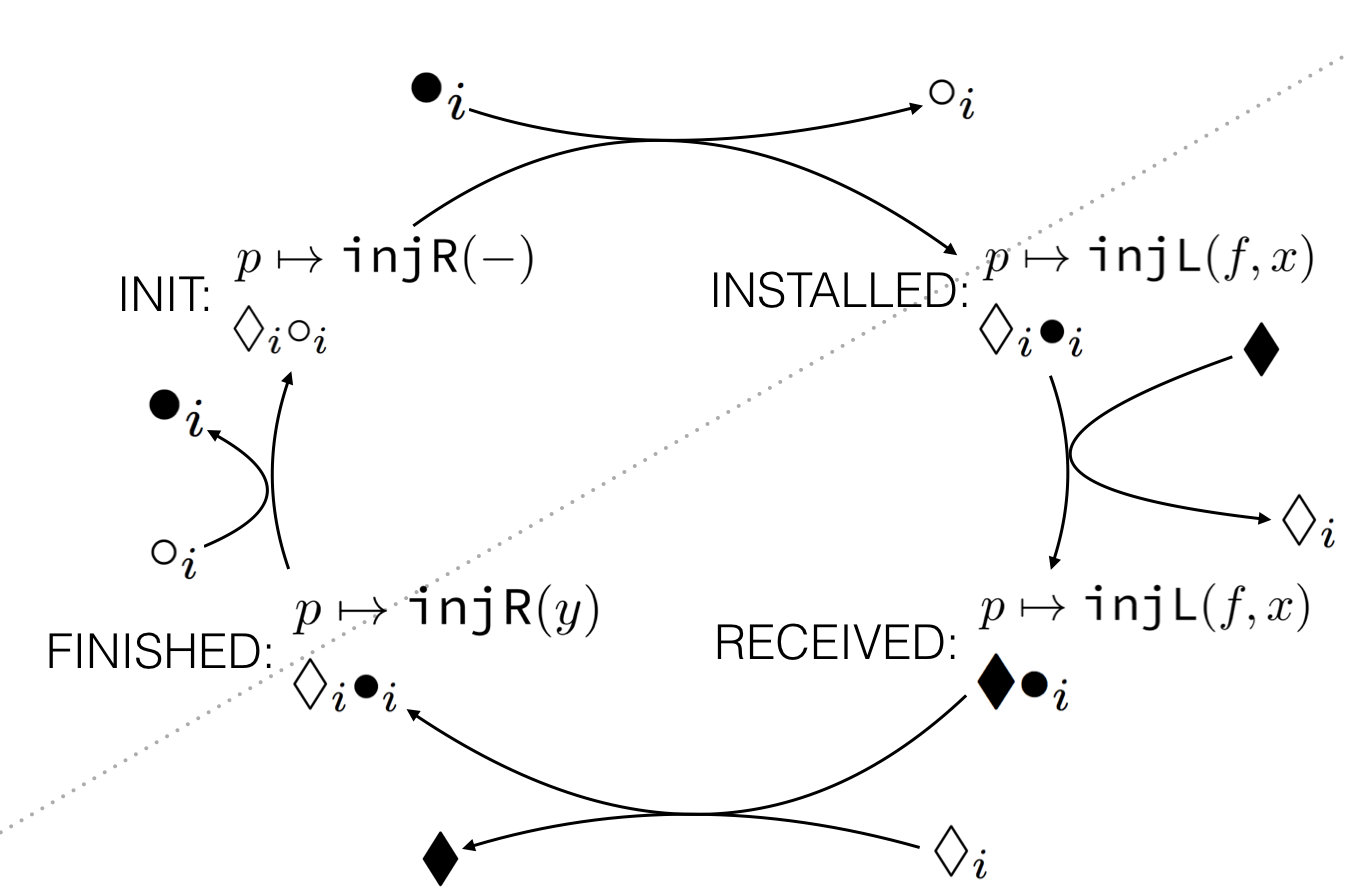
\includegraphics[width=0.5\textwidth]{helping}
  \caption{Helping protocol illustration. Note that this graph is heavily simplified to reflect how I encode protocol with bare exclusive monoids.}
\end{figure}

The black diamond is a token owned by server lock; The other three kinds of token are all tagged with i, which is similar to thread id in CaReSL’s reasoning, but in my case, it is the slot address (In some sense it is more flexible since in that way, the same thread can initiate several operations at the same time).

Here is the per-item (i.e. request slot) invariant, which have four branches.

\begin{align*}
     &\Exists y.          &&p \fmapsto[1/2] \injR(-) * \dia_i * \circ_i\\
\lor &\Exists f, x, P, Q. &&p \fmapsto[1/2] \injL(f, x) * \ownGhost{\gname}{x^{1/2}} *
                           P(x) * (\hoare{R * P(x)}{f(x)}{v.\,R * Q(x, v)}) * \kappa \mapstoprop Q(x) * \dia_i * \bullet_i\\
\lor &\Exists x.          &&p \fmapsto[1/2] \injL(-, x) * \ownGhost{\gname}{x^{1/4}} * \bdia * \bullet_i\\
\lor &\Exists x, y.       &&p \fmapsto[1/2] \injR(y) * \ownGhost{\gname}{x^{1/2}} * \kappa \mapstoprop Q(x) * Q(x, y) * \dia_i * \bullet_i
\end{align*}


Note how $f, x, P, Q$ are all hidden under existential qualification, and $Q(x)$ is saved under some constant name $\kappa$. Note how only post-condition matters to waiting client.


\end{document}
